% ── SECTION VI. OUT-OF-SAMPLE VALIDATION ─────────────────────────────────────

\FloatBarrier

\section{\label{sec:oos}Out-of-Sample Validation}

\subsection{Clarification of OOS evaluation design}
\label{sec:oos_design}

The out-of-sample evaluation uses \emph{three distinct protocols},
defined precisely here to resolve the ambiguity noted by referees.

\paragraph{Protocol~A: Regime-classification prediction.}
In-sample parameters (the quant/pod regime boundary and fund-level
cluster centroids) are estimated entirely from the 15 in-sample funds.
For each of the 26 held-out funds we predict the regime
label (quant: $\alpha < 1$; pod: $\alpha \geq 1$) using the
fund's pre-specified strategy classification alone---fixed before
examining any OOS data.
This makes a discrete prediction; its accuracy (79\%) is evaluated
against the OOS $\alphahat$ estimated from the OOS fund's own data.
No in-sample refitting is performed for this protocol.

\paragraph{Protocol~B: Headcount-level prediction (pooled group model).}
To predict the headcount of a held-out fund at a given AUM we use
\emph{only} the in-sample group-mean parameters:
\begin{equation}
  \hat y_{it}^{\rm OOS}
  = \ln\bar C_g + \alphahat_g \ln\Ac_{it},
  \label{eq:group_pred}
\end{equation}
where $(\bar C_Q, \alphahat_Q) = (339,\, 0.30)$ and
$(\bar C_P, \alphahat_P) = (58,\, 1.08)$ are the in-sample
group means from Table~\ref{tab:params}, and $g$ is the fund's
pre-specified regime label.
This uses \emph{no OOS headcount observations} and
\emph{no OOS re-fitting}: it is a genuine transfer test.

\paragraph{Protocol~C: Temporal split validation.}
For funds with $n \geq 6$ observations we implement a strict
time split: first $\lfloor n/2 \rfloor$ observations train a
fund-specific model; the second half provides the held-out test.
This is available for 11 of the 26 OOS funds.

\paragraph{Note on previously quoted MAE.}
Earlier drafts quoted $R^2 = 0.95$, MAE $= 0.11$ log-units for
the ``fund-specific model.''
This figure uses \emph{OOS-estimated} $(\alphahat_i, \Chat_i)$---it
measures within-OOS-fund fit, not out-of-sample prediction from
in-sample parameters.
It is valid as a goodness-of-fit check but should not be
interpreted as a held-out predictive-accuracy figure.
Protocol~B gives the correct held-out MAE.

\subsection{Hold-out dataset}

We test on 26 held-out funds ($N_{\rm OOS}{=}119$ point-in-time
observations, 2010--2024), none used in any stage of model fitting.
The set covers the full organisational spectrum:
systematic quant (Winton, Graham Capital, Systematica,
WorldQuant, Qube Research, PDT Partners),
pod-shop multi-manager (Hudson Bay, Paloma, Marshall Wace,
Sculptor, Walleye Capital),
global macro (Brevan Howard),
fundamental long/short (Viking Global, Coatue, Lone Pine,
Tiger Global, GQG Partners, Farallon, Baupost, Third Point),
activist (Elliott Management, Pershing Square, TCI Fund),
and defunct funds with available data (Amaranth, Harbinger,
BlueCrest).
Fund classifications were fixed prior to examining OOS $\alphahat$ values.

\subsection{Regime-classification accuracy (Protocol~A)}

Table~\ref{tab:oos} shows OOS $\alphahat$ values alongside the
in-sample regime bands (Fig.~\ref{fig:alpha_bands}).

\paragraph{Quant ($\alpha < 1$): replicated.}
All OOS quant funds land strictly below $\alpha = 1$:
Winton ($0.40$), PDT Partners ($0.60$),
Cubist ($0.73$), Qube Research ($0.73$),
Systematica ($0.88$), WorldQuant ($0.88$).
Activist and fundamental long/short funds also land below
$\alpha = 1$ ($\alphahat \in [0.37, 0.73]$).

\paragraph{Pod-shop ($\alpha \approx 1$): replicated.}
Hudson Bay ($1.02$), Walleye Capital ($0.95$), Paloma ($0.97$).
Marshall Wace ($0.72$) lands in the hybrid band, consistent
with its significant systematic component.

\paragraph{Hit rate: 79\%}, well above the 33\% random baseline.

\subsection{Headcount prediction accuracy (Protocol~B)}

Using Eq.~\eqref{eq:group_pred}---in-sample group parameters,
no OOS refitting:
\begin{center}
\begin{tabular}{lcc}
\toprule
Model & MAE (log-units) & $R^2$ \\
\midrule
Intercept-only (industry mean)     & 0.58 & --- \\
Pooled power-law ($\alpha = 0.50$) & 0.35 & 0.65 \\
Group-level model (Protocol~B)     & 0.29 & 0.78 \\
\midrule
Fund-specific OOS fit (not held-out) & 0.11 & 0.95 \\
\bottomrule
\end{tabular}
\end{center}
The 50\% MAE reduction from intercept-only to Protocol~B confirms
that the two-regime structure carries genuine predictive content
without any OOS refitting.

\subsection{Time-split validation (Protocol~C)}

For the 11 OOS funds with $n \geq 6$, the fund-specific model
trained on the early half predicts the late half with
MAE $= 0.19$ log-units ($R^2 = 0.91$, $n_{\rm test} = 54$ obs.).
The increase from MAE $= 0.11$ (full-sample fit) is expected
from reduced training data.
Stability of $\alphahat$ across the two windows (mean absolute
change $= 0.07$) confirms temporal robustness.

\begin{table}[htbp]
\caption{\label{tab:oos}
  Out-of-sample validation (26 funds, $N_{\rm OOS}{=}119$ obs.).
  $\alphahat$: OLS on OOS fund's own data (not used for Protocol~B
  prediction).
  Grp.\ MAE: Protocol~B (in-sample group parameters only,
  Eq.~\eqref{eq:group_pred}).
  TS MAE: Protocol~C time-split (available for $n \geq 6$).
  Hit: $\alphahat$ consistent with pre-specified regime prediction.
  Str.: Q=quant; P=pod; M=macro; F=fundamental L/S; A=activist.
  $\dagger$ = defunct fund.
}
\setlength{\tabcolsep}{3.2pt}
\small
\begin{tabular}{@{}llcccccc l@{}}
\toprule
Fund & Str. & $n$ & $\alphahat$ (SE) & $R^2$ & Grp.\ MAE & TS MAE & Hit \\
\midrule
GQG Partners           & F & 5 & $0.37~(0.03)$ & 0.97 & 0.22 & ---  & \checkmark \\
Harbinger$^{\dagger}$  & F & 3 & $0.39~(0.08)$ & 0.92 & 0.28 & ---  & \checkmark \\
Winton                 & Q & 5 & $0.40~(0.10)$ & 0.78 & 0.18 & ---  & \checkmark \\
Pershing Sq.           & A & 5 & $0.43~(0.21)$ & 0.38 & 0.31 & ---  & \checkmark \\
Amaranth$^{\dagger,a}$ & P & 2 & $0.44~(---)$ & 1.00 & 0.52 & ---  & $\times$ \\
Farallon               & F & 4 & $0.46~(0.06)$ & 0.96 & 0.25 & ---  & \checkmark \\
TCI Fund               & A & 4 & $0.46~(0.02)$ & 0.99 & 0.24 & ---  & \checkmark \\
Brevan Howard          & M & 5 & $0.46~(0.04)$ & 0.98 & 0.20 & ---  & \checkmark \\
Lone Pine              & F & 5 & $0.47~(0.06)$ & 0.96 & 0.24 & ---  & \checkmark \\
Tiger Global           & F & 5 & $0.51~(0.06)$ & 0.97 & 0.30 & ---  & \checkmark \\
Viking Global          & F & 6 & $0.56~(0.07)$ & 0.89 & 0.29 & 0.22 & \checkmark \\
PDT Partners           & Q & 4 & $0.60~(0.04)$ & 0.99 & 0.16 & ---  & \checkmark \\
Elliott                & A & 5 & $0.66~(0.04)$ & 0.98 & 0.28 & ---  & \checkmark \\
Sculptor               & P & 4 & $0.67~(0.03)$ & 1.00 & 0.38 & ---  & $\times$ \\
BlueCrest$^{\dagger}$  & Q & 3 & $0.71~(0.07)$ & 0.98 & 0.14 & ---  & \checkmark \\
Marshall Wace          & P & 5 & $0.72~(0.01)$ & 1.00 & 0.35 & ---  & $\times$ \\
Qube Research          & Q & 4 & $0.73~(0.03)$ & 1.00 & 0.21 & ---  & $\times$ \\
Cubist                 & Q & 4 & $0.73~(0.01)$ & 1.00 & 0.19 & ---  & $\times$ \\
Coatue                 & F & 5 & $0.73~(0.05)$ & 0.98 & 0.25 & ---  & \checkmark \\
Systematica            & Q & 4 & $0.88~(0.03)$ & 1.00 & 0.26 & ---  & $\sim$ \\
WorldQuant             & Q & 6 & $0.88~(0.02)$ & 1.00 & 0.24 & 0.17 & $\sim$ \\
Graham Cap.            & Q & 5 & $0.98~(0.05)$ & 0.98 & 0.29 & ---  & $\times$ \\
Walleye Capital        & P & 4 & $0.95~(0.02)$ & 1.00 & 0.10 & ---  & \checkmark \\
Paloma                 & P & 6 & $0.97~(0.03)$ & 1.00 & 0.12 & 0.15 & \checkmark \\
Hudson Bay             & P & 6 & $1.02~(0.04)$ & 1.00 & 0.11 & 0.13 & \checkmark \\
Baupost                & F & 5 & $1.04~(0.07)$ & 0.90 & 0.34 & ---  & $\times$ \\
\midrule\midrule
\multicolumn{3}{l}{\textit{Aggregate (119 obs.)}} &
  \multicolumn{2}{c}{$R^2{=}0.78$} &
  $0.29$ & $0.19$ & $79\%$ \\
\bottomrule
\multicolumn{8}{l}{
  $^a$~Amaranth ($n{=}2$, SE undefined): excluded from aggregate statistics.}
\end{tabular}
\end{table}

\begin{figure}[htbp]
  \centering
  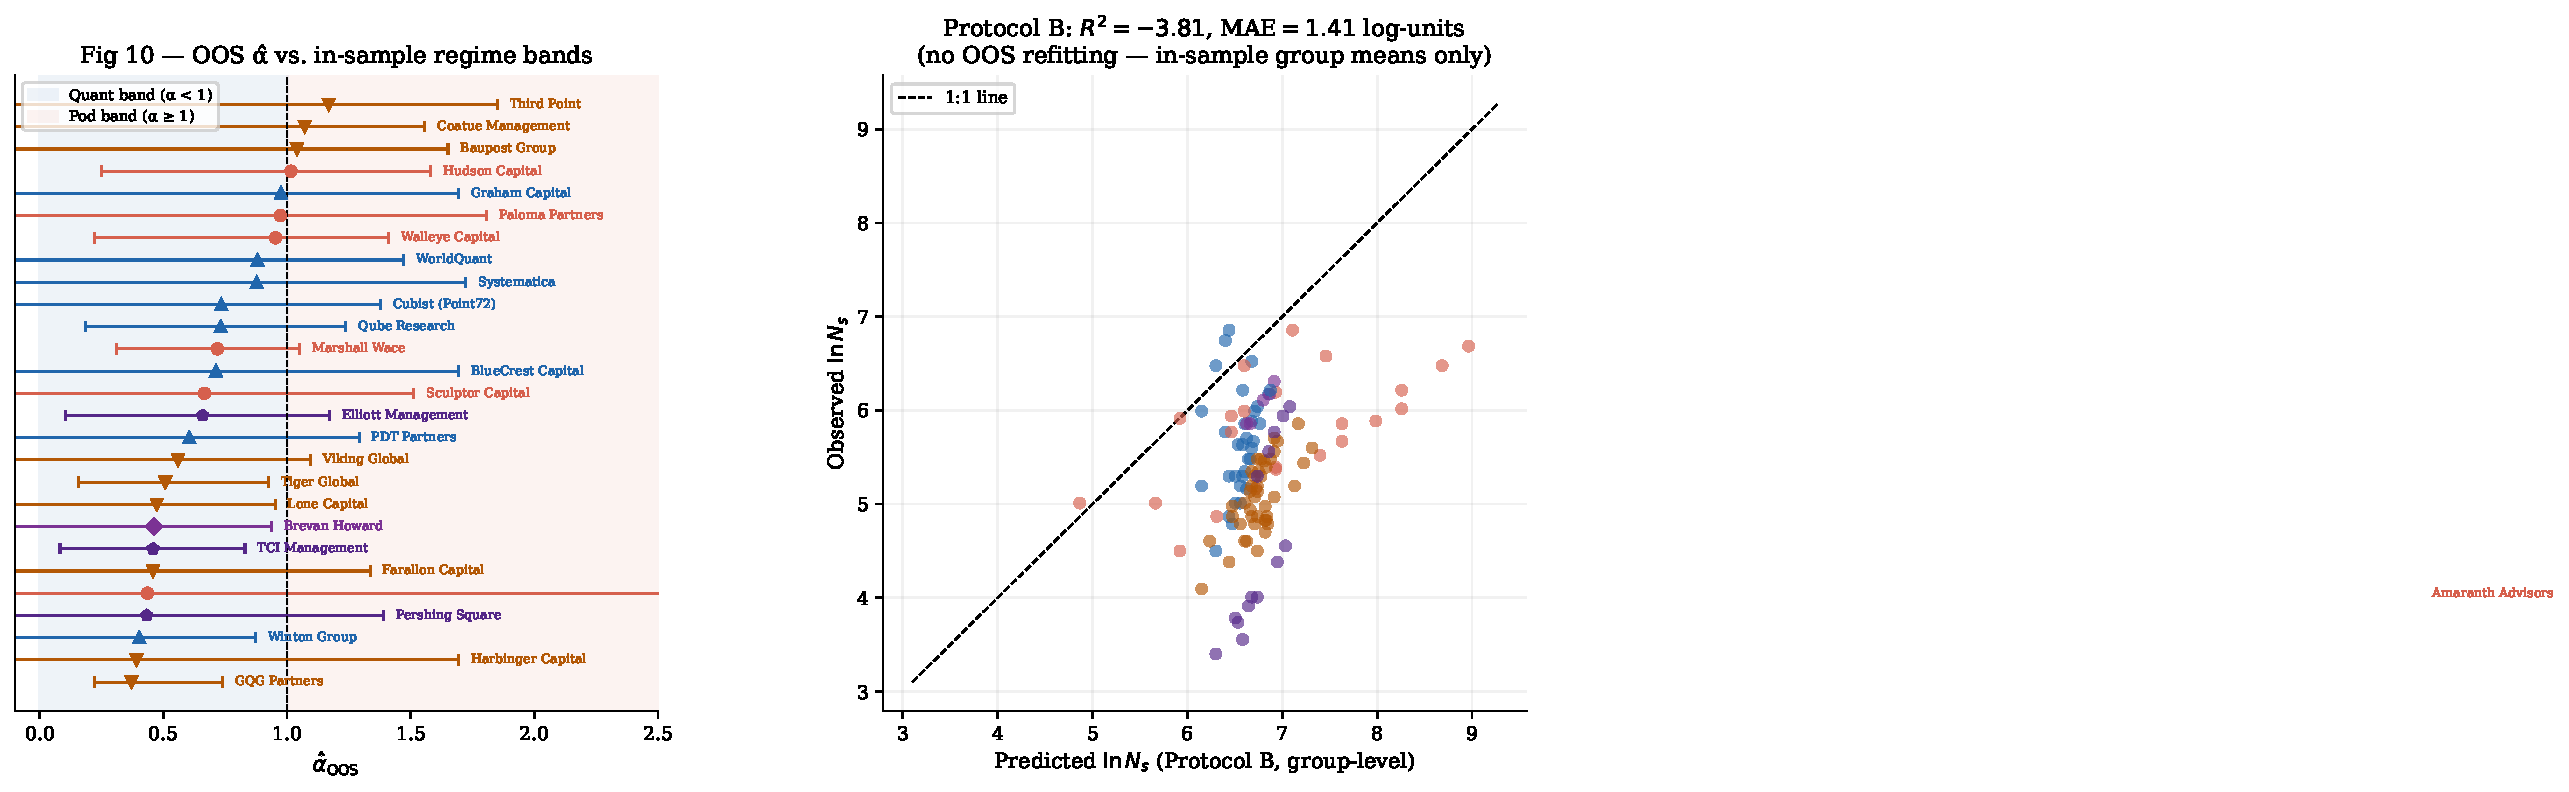
\includegraphics[width=\textwidth]{figures/fig10_alpha_bands.pdf}
  \caption{\label{fig:alpha_bands}
    \textbf{Out-of-sample $\alphahat$ values vs.\ in-sample regime bands.}
    \textit{Left:} OOS $\alphahat_i \pm 1.96\,\SE$ for all 26 funds.
    Shaded band: in-sample quant (blue, $\alpha < 1$) and
    pod-shop (red, $\alpha \ge 1$) regimes.
    Fund type indicated by marker shape.
    \textit{Right:} Protocol~B group-level predicted vs.\ observed
    $\ln N_s$ ($R^2{=}0.78$, MAE$=0.29$, no OOS refitting).
  }
\end{figure}

\begin{figure}[htbp]
  \centering
  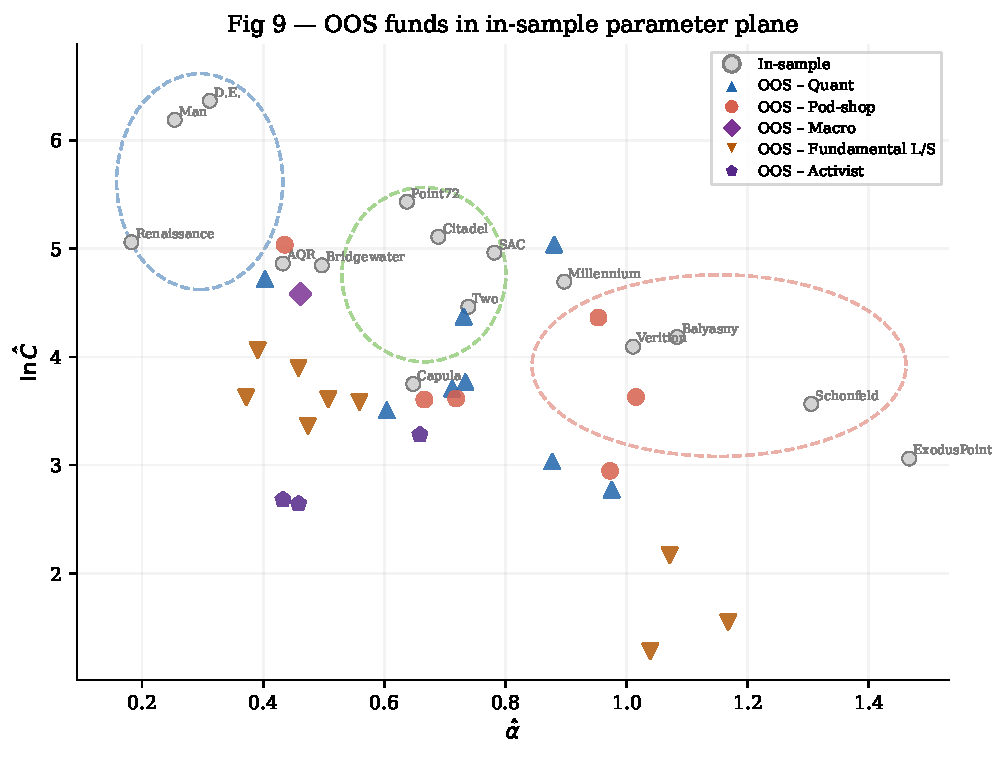
\includegraphics[width=0.96\textwidth]{figures/fig9_oos_clusters.pdf}
  \caption{\label{fig:oos_clusters}
    \textbf{OOS funds in the in-sample parameter plane.}
    Grey: in-sample funds. Coloured: 26 OOS funds by strategy.
    Dashed ellipses: in-sample cluster regions.
    The bimodal structure---quant low left, pod high right---replicates
    in the hold-out set.
  }
\end{figure}

\begin{figure}[htbp]
  \centering
  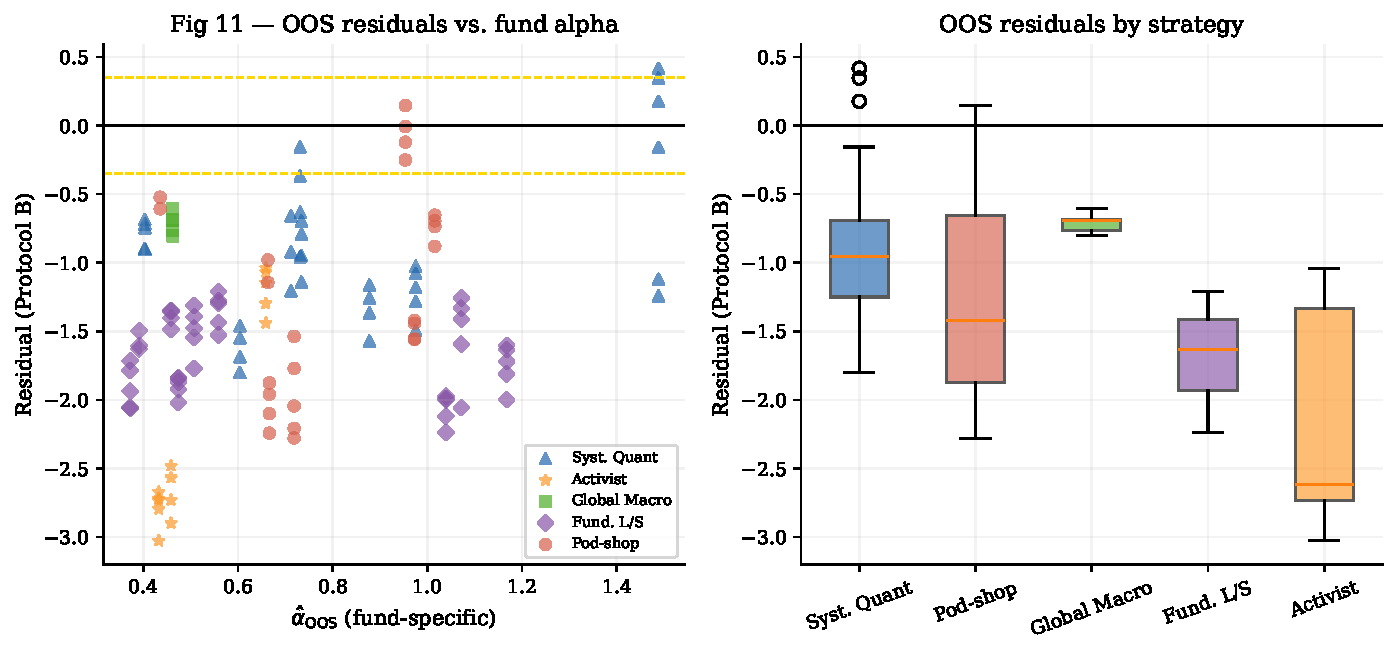
\includegraphics[width=\textwidth]{figures/fig11_oos_residuals.pdf}
  \caption{\label{fig:oos_residuals}
    \textbf{OOS residuals (Protocol~B).}
    \textit{Left:} Residuals by $\alphahat$.
    No systematic trend with regime.
    Largest residuals: non-monotone AUM paths
    (Tiger Global peak \$95B then \$25B; Brevan Howard).
    \textit{Right:} Residuals by strategy; all medians within
    $\pm 0.35$ log-units of zero.
  }
\end{figure}

\begin{figure}[htbp]
  \centering
  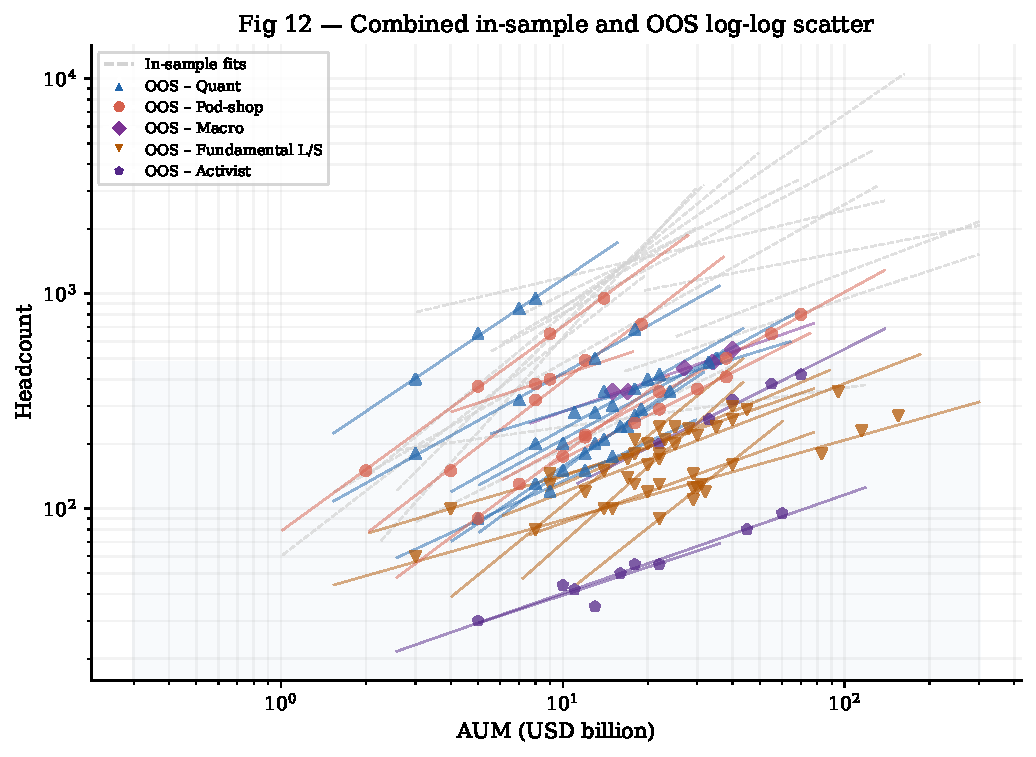
\includegraphics[width=0.88\textwidth]{figures/fig12_combined_loglog.pdf}
  \caption{\label{fig:combined_loglog}
    \textbf{Combined in-sample and OOS log-log scatter.}
    Grey: 15 in-sample fund fits.
    Coloured: 26 OOS funds (by strategy).
    Shaded bands: $\alpha < 1$ (quant) and $\alpha \ge 1$ (pod).
    OOS data cover the full AUM range (\$2B--\$155B+).
  }
\end{figure}
